\graphicspath{{chapters/notes/09/images/}}
\chapter{Extracellular vesicles}
\emph{Introduction to Extracellular vesicles as disease biomarker carriers in the circulation of patients}

We will be trying to answer three main questions: what are EVs? Why are we interested in them? How can we use them to study cancer? (or any other disease)

\section{Definition}
“Extracellular vesicles are membrane-enclosed nanoscale particles released from essentially all prokaryotic and eukaryotic cells that carry proteins, lipids, RNA and DNA.”
\\
The outside layer is made of the lipidic membrane of the cells from which the vesicles were originated.
The content can vary: RNAs of different length, DNA, proteins. They also come from the cell that originated the vesicles.\\
On the membrane there are proteins that are able to to interact with he immune system, receptors, adhesion molecules and tetraspanins (they span the membrane four times, and are markers, or recognition proteins of the vescicle).
Figure \ref{fig:ev1} represents all the main components of a vesicle.
\begin{figure}[H]
    \centering
    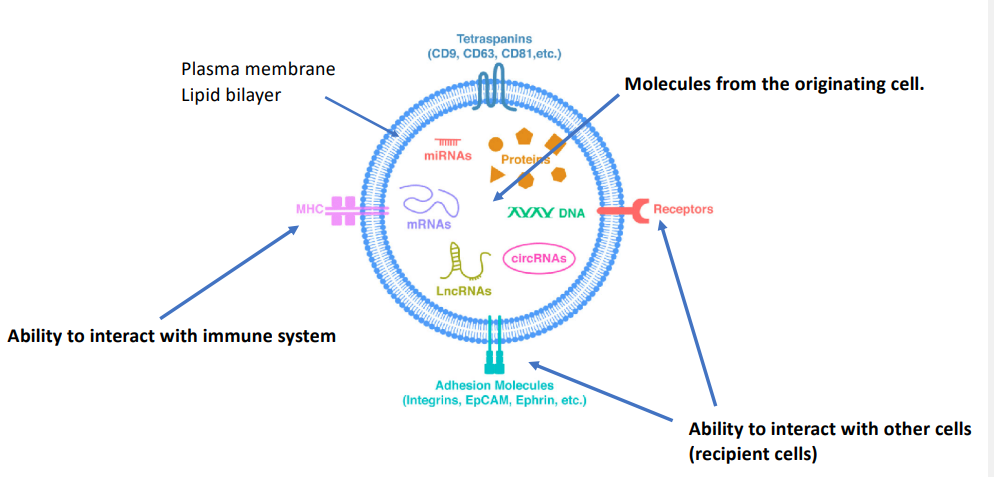
\includegraphics[width=0.5\textwidth]{ev1.png}
    \caption{Sketch representing the main components of an EV.}
    \label{fig:ev1}
\end{figure}

\section{Characterization}
Extracellular vesicles are very different from each other.
Especially in older studies, each research group used to study EVs from a certain site and gave the EVs a specific name (for examples, EVs from the prostate were called \textit{prostatosomes}, from a tumor sample were called \textit{oncosomes} and so on).
\\
A consortium was created to make some order in the nomenclature and which are the parameters to characterize and study them.

\subsection{Size}
The smallest vesicles are the microvesicles (100 -1000 nm), then we find the exosomes (50 - 150nm), finally the apoptotic EVs and apoptotic bodies (100-5000 nm). Note that the categories overlap, there's no clear cut. Exomeres could represent a new class of EV with no lipid bilayer and are 30-50nm long.

\subsection{Origin}
Exosomes come from the endocytic pathway, microvesicles and apoptotic bodies from the plasma membrane.
\\
Microvesicles come directly from the membrane of the cell, while the exosomes come from the multivescivular body, which contains the intraluminal vesicles, as shown in panel a) of figure \ref{fig:origin}.
\\
Apoptotic bodies instead are the result of cell death. In the experiment performed in panel b) of figure \ref{fig:origin}, the researchers induced apoptosis using different methods and the vesicles had different sized.

\begin{figure}
\begin{tabular}{cc}
  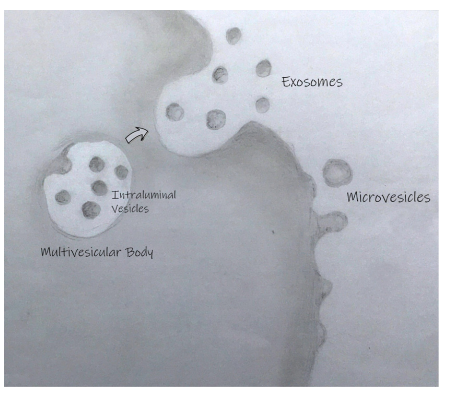
\includegraphics[width=65mm]{origin1} &   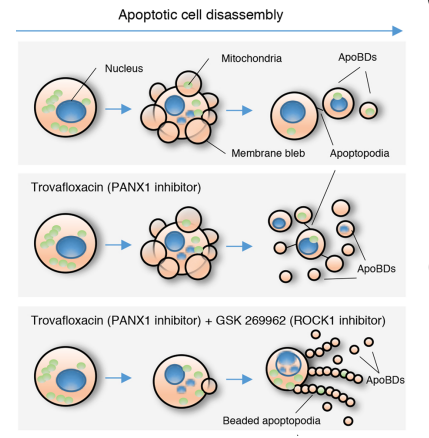
\includegraphics[width=65mm]{origin2} \\
(a) Origin of exosomes and microvesicles & (b) Origin of apoptotic body \\[6pt]

\end{tabular}
\caption{caption}
\label{fig:origin}
\end{figure}

The main steps in the origin of exosomes, the EVs of main interest, are:
\begin{itemize}
\item Endocytosis: the cell either capture everything in the ECM, or the substrate is selected by receptors.
\item Formation of early and late endosomes: lysosomes are organelles which go through a process of maturation, in the late endosomes enzymes complete the packaging of the substrate.
\item Formation of multi Vesicular bodies: Multivesicular bodies contain intralumenal vesicles, the precursors of the exosomes.
\end{itemize}

\subsection{Content}
Exosomes and microvescicles mainly carry proteins and nucleic acids (mRNA, miRNA and other non-coding RNAs). But which type of nucleic acids? The vesicles are really smalls and cannot contain big fragments of DNA. Further studies however proved the presence of longer, protein coding transcripts. A lot of RNA transcripts have important regulatory functions (like miRNA, circRNA etc).
\\
Apoptotic bodies instead are the entire representation of the cell's cytoplasm. They have an equal representation of the cell content, whereas for exosomes there's an active process of selection of the cargo.
\\
How does the cell select the cargo?
\begin{itemize}
\item Abundant RNA
\item Fragmentation
\item Particular sequence motifs
\item Unique secondary structures
\item RNA modification (eg.mRNA uridylation)
\end{itemize}


\section{The importance of EVs}
Main reason: each EV carries information about its cell of origin and its putative function! What can be the function of the EVs, how does it act in presence of other recipient cells, what's the effect on other cells?

\subsection{Role in cancer}
In cancer, EVs have important functions. In prostate cancer it has been shown that exosomes are able to modulate the immune system, by changing the preferential maturation of the cells of the immune systems. They aid in the proliferation of endothelial cells, in stromal fibroblast differentiation, creating population that are pro/anti tumorigenic. They act on the remodeling of ECM, which is extremely important for metastasis, as EVs provide for a way for cells to harbor to a different substrate and create metastatic sites (especially for bone cancer). An example of how exosomes can boost metastasis is reported in figure \ref{fig:cancer1}.

\begin{figure}[H]
    \centering
    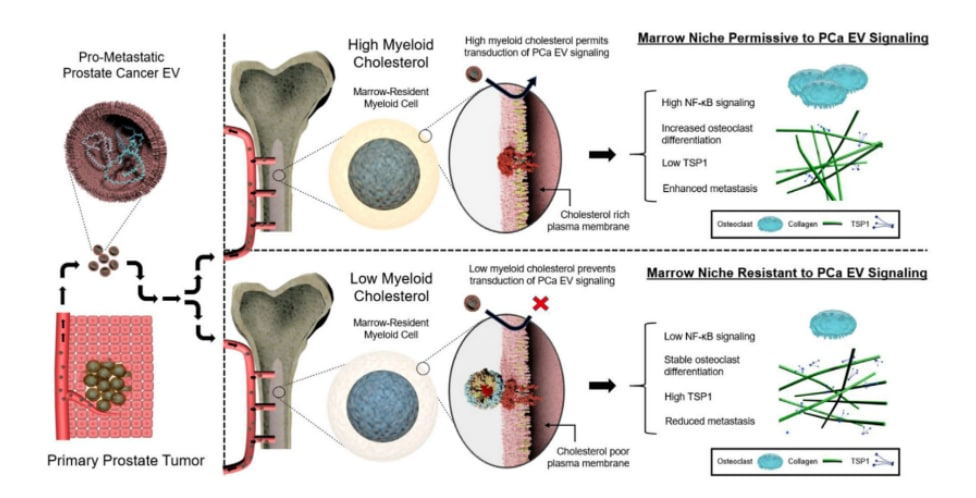
\includegraphics[width=0.5\textwidth]{cancer1.png}
    \caption{Prostate cancer extracellular vesicles mediate intercellular communication with bone marrow cells and promote metastasis in a cholesterol-dependent manner.\textit{ Stephen E. Henrich, JExtracell Vesicles. 2020}.
    \\
    Exosomes from prostate cancer travel in the body, arrive to the bone and boost metastasis. }
    \label{fig:cancer1}
\end{figure}


\section{How can we use them to study cancer? (or any other disease)}
Use liquid biopsy as a novel tool for cancer detection and monitoring. By just drawing some blood, in a serial matter, we can retrieve a lot of EVs, coming from all of the tissues of the body, including the cancer cells.
\\
In the same tumor there could be different populations, each harboring different mutations and having different proliferation rates. They respond in different ways to therapies.
\\
In the bloodstream we have cells coming from the tumor, free cDNA, EVs and ribolipoproteins. We can perform the analysis of the lquid biopsy with a Multi-analyte approach: using different molecules/analysis (es. DNA, RNA) to detect tumor related signal.
\\

\begin{figure}[H]
    \centering
    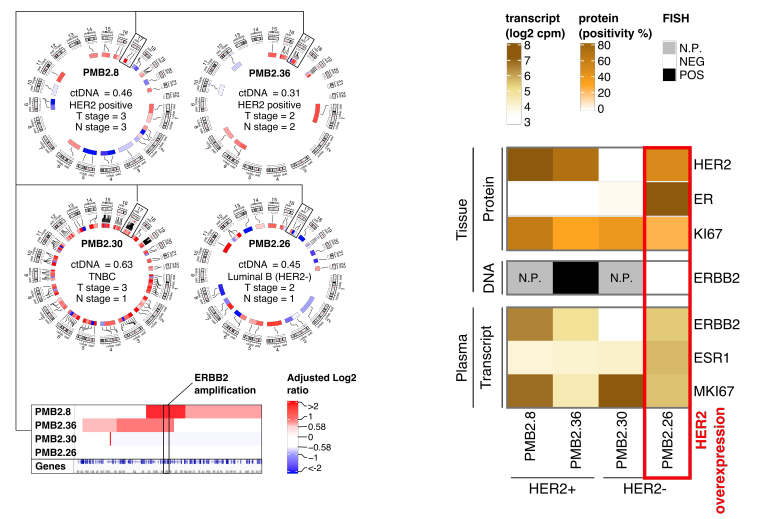
\includegraphics[width=0.5\textwidth]{cancer2.png}
    \caption{4 Breast cancer patients. On the left:  Whole Exome Sequencing of cfDNA from plasma. }
    \label{fig:cancer2}
\end{figure}

Breast cancer usually stratifies in different subtype and one of the main molecular feature is the presence of hormon receptors, in particular the one expressed by HER2.
Two patients that were HER2 positive and two patients HER2 negative. The two positive patients were confirmed by high protein level, but one of the negative patients has a signal for the protein, but no amplification (performed with FISH). At the end, the clinicians classified this ambiguous patient as... ambiguous.
\\
By integrating the RNA form the EVs, for the HER2 positive we have high expression of ERBB2 (concordant with the previous results), but also for a HER2- patient. This is concordant witht he immuno istochemistry but not by FISH. Why? The regulationof HER2 is not only regulated by the amplification, but also by over-expression.
\\
If we only perform the geneic analysis we would have missed important info, because with EVs we were able to identify over-expression even in abscense of amplification.

\subsection{Tracking tumor signal in serial samples}
Serial approach: tracking the signal of different biomarkers in time. Es: tracking response to a drug treatment. In this

Sequence/perform digital PCR on the saples from the blood and follow the biomarkers in time, to discover how well the patient is responding to the treatment.

\subsection{Different EVs isolation methods}
